\section*{Stationskarte: \ref{sec:kommunikation} \nameref{sec:kommunikation}}

\margininfo{}
\begin{multicols}{2}
\subsection*{Material-Liste}
\begin{itemize}
  \item Arduino Uno mit Breadboard
  \item Pushbottum
  \item Widerstand (10k$\Ohm$)
\end{itemize}


\vfill\null 
\columnbreak

\subsection*{Versuchsaufbau}

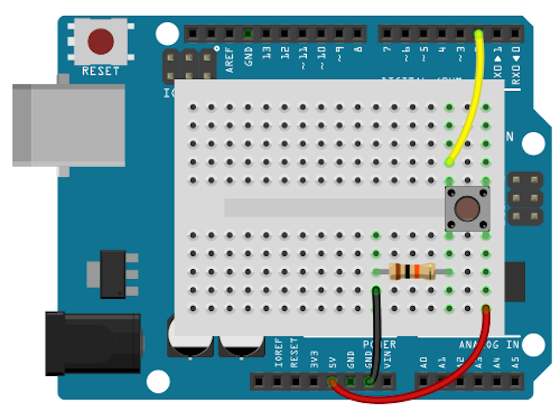
\includegraphics[width=0.5\textwidth]{Kapitel1/Bilder/digitalreadserial2}
\end{multicols}




\section*{Stationskarte: \ref{sec:lm35} \nameref{sec:lm35}}

\margininfo{Achte darauf, dass du den LM35 richtig einbaust. Sollte er sich erwärmen, musst du die Stromversorgung zum Arduino sofort unterbrechen, und den Aufbau deiner Schaltung überprüfen!}
\begin{multicols}{2}
\subsection*{Material-Liste}
\begin{itemize}
  \item Arduino Uno mit Breadboard
  \item Temperatur Sensor LM35
  \item 3 Projekt-Kabel
\end{itemize}


\vfill\null 
\columnbreak

\subsection*{Versuchsaufbau}

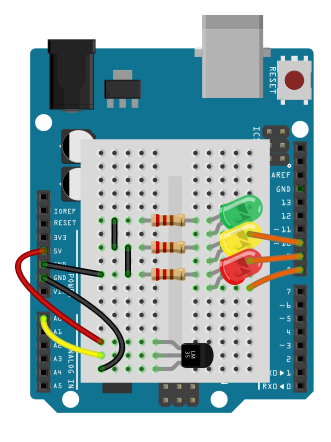
\includegraphics[width=0.5\textwidth]{Kapitel2/Bilder/temperatursensor}
\end{multicols}


\section*{Stationskarte: \ref{sec:lichtsensoren} \nameref{sec:lichtsensoren}}

\margininfo{}
\begin{multicols}{2}
\subsection*{Material-Liste}
\begin{itemize}
  \item Arduino Uno mit Breadboard
  \item LDR (Photozelle)
  \item Widerstand (muss bestimmt werden)
  \item Multimeter
  \item 3 Projekt-Kabel
\end{itemize}

\subsection*{Übersicht Material}

\vfill\null 
\columnbreak

\subsection*{Versuchsaufbau}

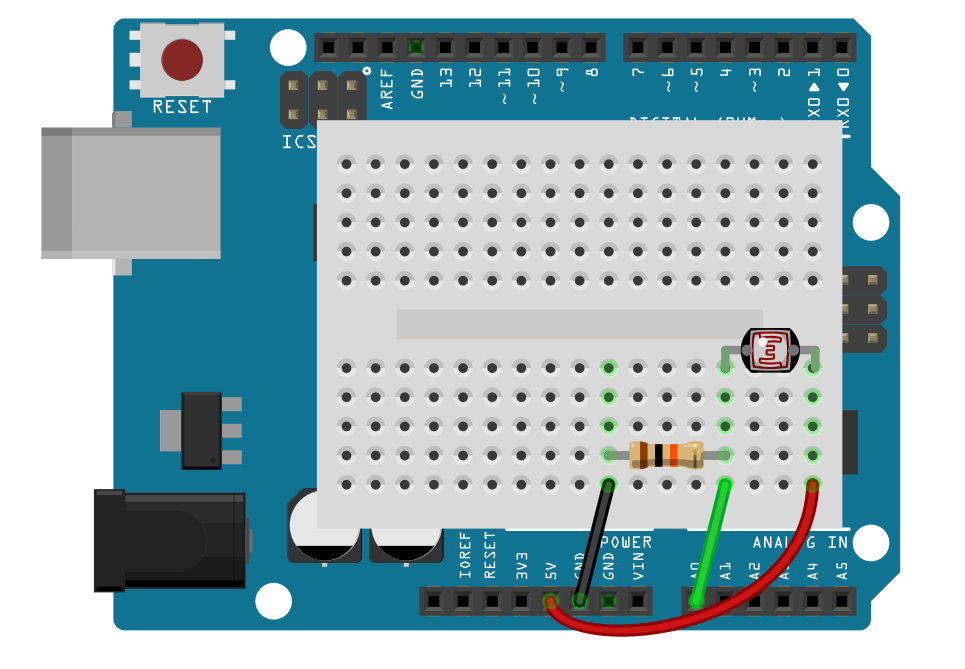
\includegraphics[width=0.5\textwidth]{Kapitel2/Bilder/LDR_bb}
\end{multicols}

\section*{Stationskarte: \ref{sec:reflex} \nameref{sec:reflex}}

\margininfo{}
\begin{multicols}{2}
\subsection*{Material-Liste}
\begin{itemize}
  \item Arduino Uno mit Breadboard
  \item cny70 (Reflexoptokoppler)
  \item Widerstände ($220\Ohm$ und $10k\Ohm$)
  \item 3 Projekt-Kabel
\end{itemize}

\subsection*{Übersicht Material}

\vfill\null 
\columnbreak

\subsection*{Versuchsaufbau}

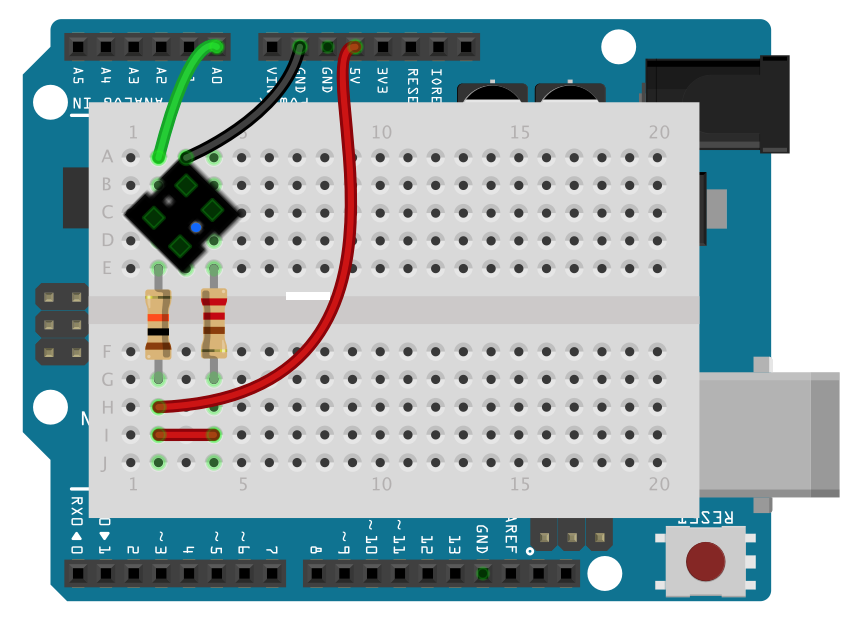
\includegraphics[width=0.5\textwidth]{Kapitel2/Bilder/cny70bb}
\end{multicols}


\section*{Stationskarte: \ref{sec:ultra} \nameref{sec:ultra}}

\margininfo{}
\begin{multicols}{2}
\subsection*{Material-Liste}
\begin{itemize}
  \item Arduino Uno mit Breadboard
  \item Untraschall Sensor
  \item 3 Projekt-Kabel
\end{itemize}

\subsection*{Übersicht Material}

\vfill\null 
\columnbreak

\subsection*{Versuchsaufbau}

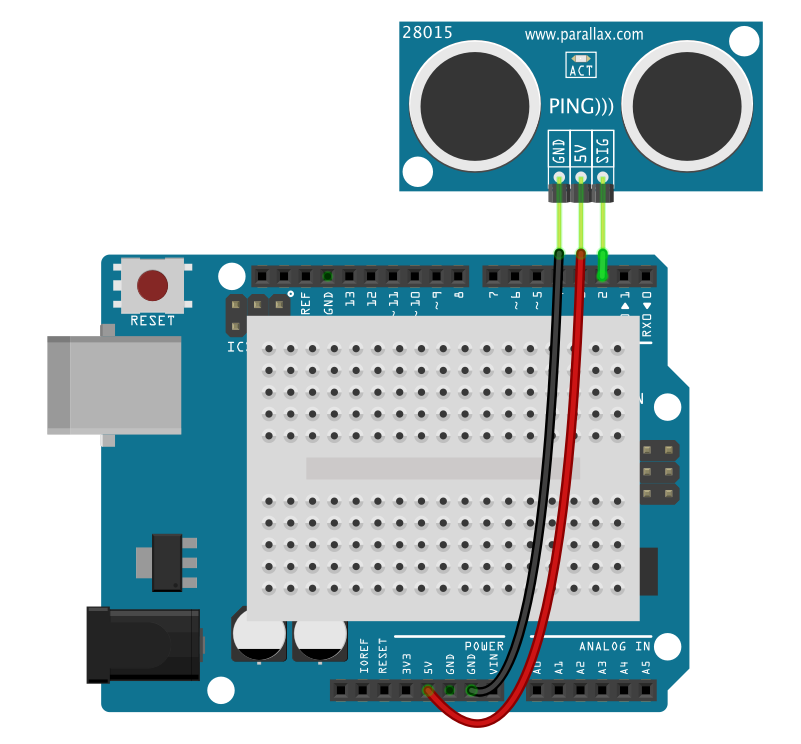
\includegraphics[width=0.5\textwidth]{Kapitel2/Bilder/ping}
\end{multicols}

\section*{Stationskarte: \ref{sec:UmweltSensoren} \nameref{sec:UmweltSensoren}}

\margininfo{}
\begin{multicols}{2}
\subsection*{Material-Liste}
\begin{itemize}
  \item Arduino Uno mit Breadboard
  \item DH11 (Temperatur und Feuchtigkeit)
  \item Widerstand ($10k\Ohm$)
  \item 4 Projekt-Kabel
\end{itemize}

\subsection*{Übersicht Material}

\vfill\null 
\columnbreak

\subsection*{Versuchsaufbau}

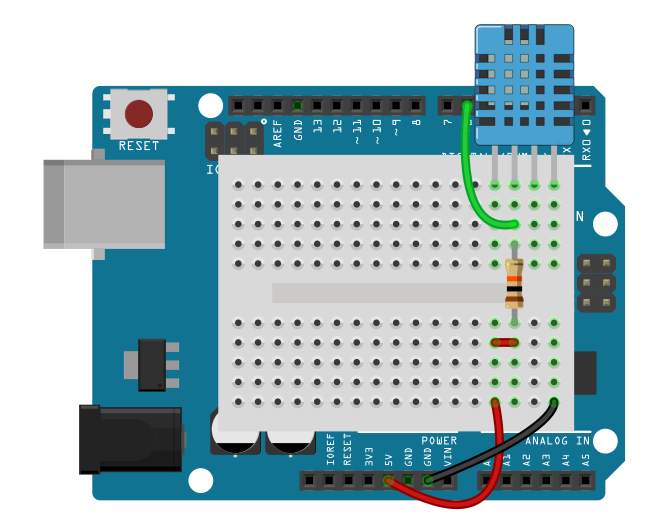
\includegraphics[width=0.5\textwidth]{Kapitel2/Bilder/dh11test}
\end{multicols}

